%!TEX root = thesis.tex

%time planning—having a Gantt chart is probably a better idea then just a list;

\section{Planning}
\label{chap:planning}

This chapter provides an overview of the deadlines for the thesis, ranging from the start of the thesis on November 10\textsuperscript{th}, 2015 to the final deadline on June 20\textsuperscript{th}, 2016. Based on these deadlines a planning has been made, which breaks down the total workload into thirteen parts. A GANTT chart is presented as a graphical presentation of the thesis planning (Figure \ref{fig:GANTT}).

\begin{figure}
	\centering
	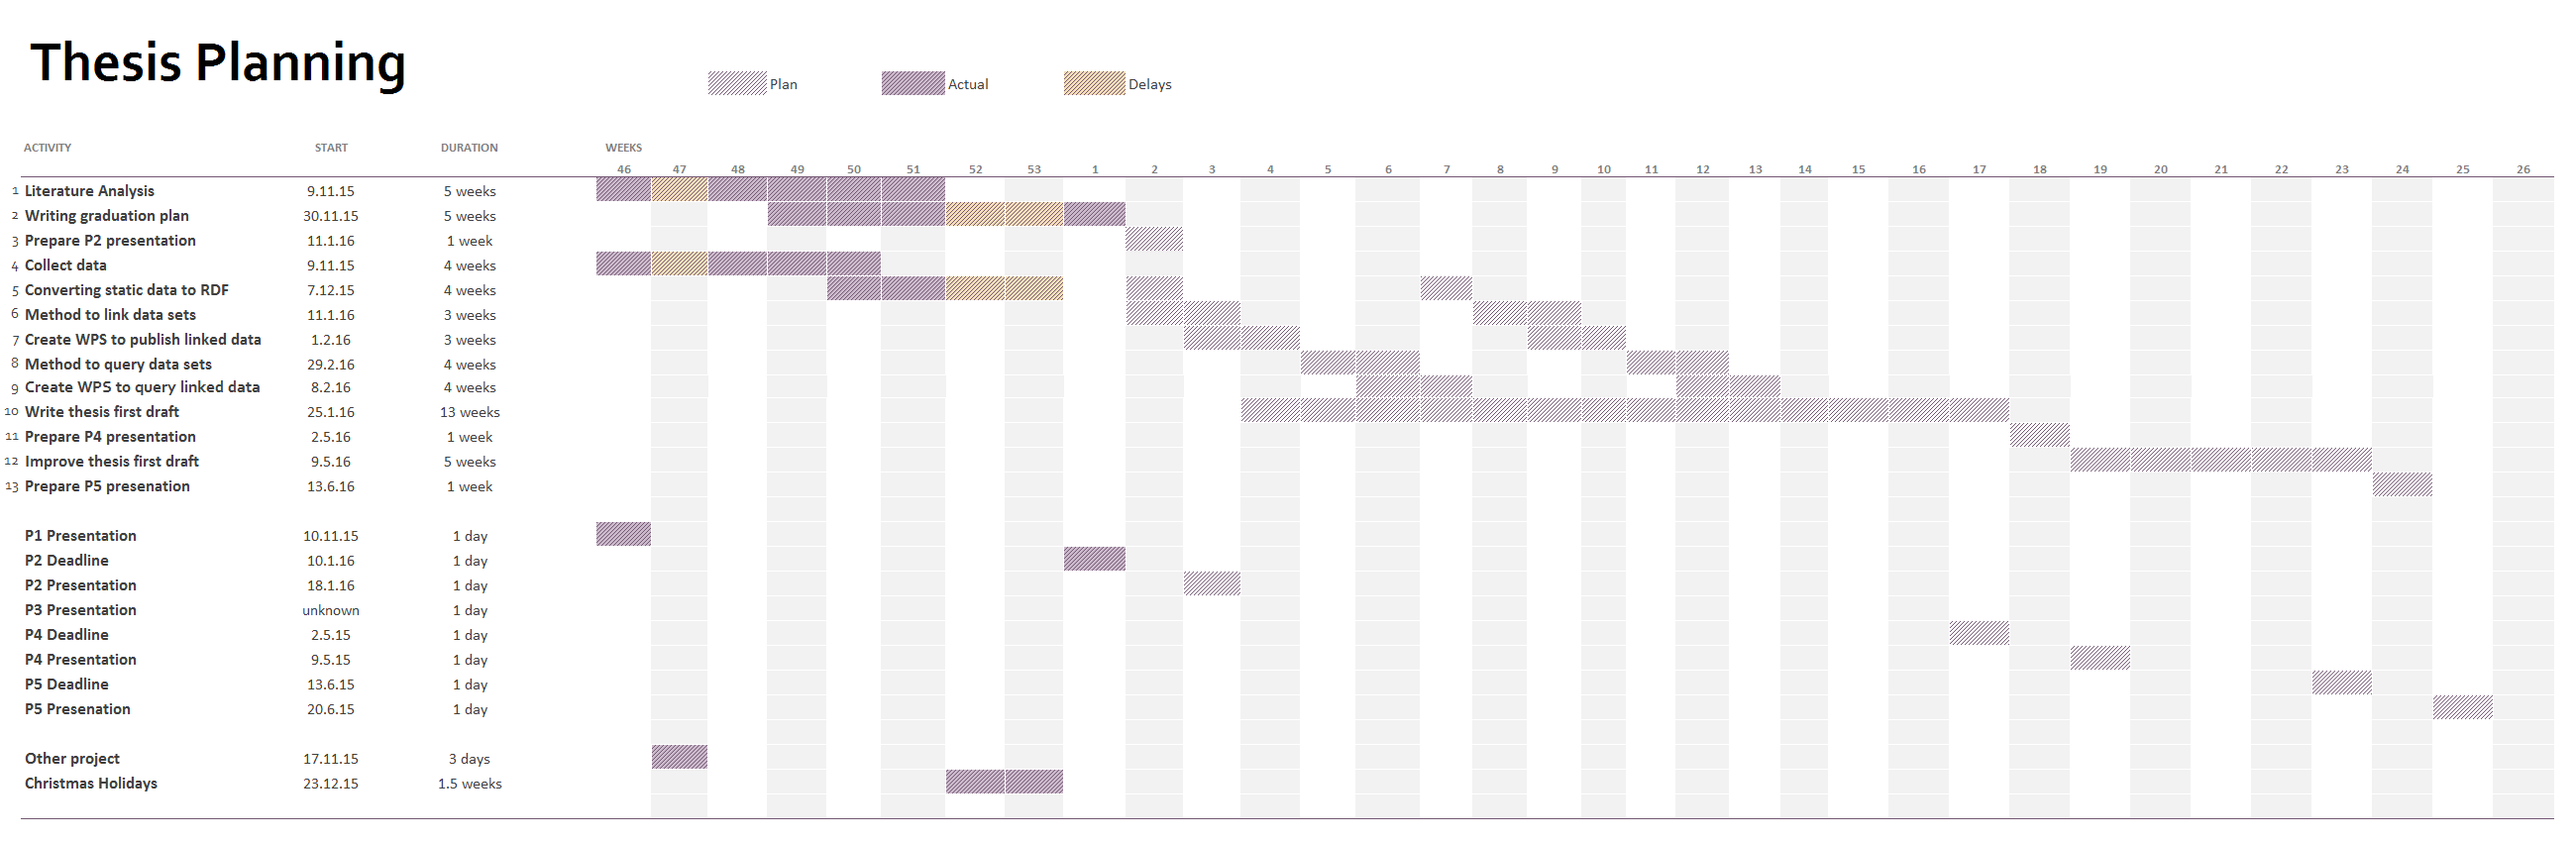
\includegraphics[width=1.5\linewidth, angle=90]{figs/GANTT-chart.png}
	\caption{GANTT chart showing the planning of the thesis}
	\label{fig:GANTT}
\end{figure}

\subsection{Deadlines}
For the planning of the thesis a number of deadlines are import. At 5 moments in time the status of the thesis has to be presented and at three of these moments it is required to hand in a report. The five deadlines are referred to as P1 to P5 in the graduation manual. P1 took place on November 10\textsuperscript{th}, 2015. The general idea for the thesis was presented here and a number of students and staff was present to provide feedback. This document is part of the deliverables for P2. At P2 the research proposal for the thesis needs to be handed in. This contains the research question, its relevance, a literature analysis of related work, a description of the methods, a planning and an overview of the tools and data that will be used. The research proposal is due January 11\textsuperscript{th}, 2016. The P2 presentation is scheduled on January 18\textsuperscript{th}, 2016. Preliminary results are presented at P3, for which the date is still unknown. The P4 presentation will be between May 9\textsuperscript{th} and May 20\textsuperscript{th}, 2016. This is the deadline for presenting the first draft of the thesis report. The deadline for handing the first draft is a week prior to the P4 presentations. The final deadline (P5) will be between the 20\textsuperscript{th} of June and the 1\textsuperscript{st} of July, 2016. The thesis outcomes will be presented afterwards.

\subsection{GANTT}
Figure \ref{fig:GANTT} shows the planning as a GANTT chart. The first six weeks were mainly focused on the preparations for writing the thesis. A literature analysis and the data collection gave insights in the current state-of-the-art of the sensor web and helped defining the research question. After P2 the work of the thesis is organised in two iterations. This way earlier work can be revisited after the first iteration to either improve it or to make changes due to unforeseen issues. Throughout the process every step will be documented right away, instead of scheduling a number of weeks before P4 to write the complete first draft of the thesis. Four weeks before the P4 deadline have also been left mostly empty to accommodate for any delays or a potential third iteration if necessary. Between P4 and P5 there is a month to improve the first draft of the thesis based on feedback.     

